\subsection{Test Introduction}
Given we are working in a \emph{mesh} network, in which nodes may join
and leave frequently and without coordination, an interesting problem
is how the routing protocol handles the sudden loss of one of its
routes. From the point of view of a user the most important factor in
this scenario is the time window in which he is cut off from the
network.

This is the rationale behind the following test in which we measured the
convergence time of \batman\ and \olsr\ when subjected to a forced
link removal.

\subsection{Topology}
 The topology of the network is the one depicted in
Picture~\ref{pic:LayoutConvergence} . The laptops are disposed in a
diamond shaped topology with the \emph{source} and \emph{sink} nodes
at the boundaries. The node 10.0.0.66 acts as \emph{preferred} path
from the \emph{source} to the \emph{sink}, while the host 10.0.0.68 works
as \emph{auxiliary} node, to be chosen when the primary route falls.

\Picture{images/convergence}
        {.90\columnwidth}
        {Configuration with single direct link}
        {pic:LayoutConvergence}

The \emph{iptables} configuration we use to setup such a topology is
the following:

\begin{itemize}
\item On 10.0.0.65 (source):

\begin{verbatim}
iptables -A INPUT -m mac --mac-source $(sinkMAC) -j DROP;
\end{verbatim}

\item On 10.0.0.66 (preferred)
\begin{verbatim}
iptables -A INPUT -m mac --mac-source $(preferredMAC) -j DROP;
\end{verbatim}

\item On 10.0.0.68 (auxiliary)
\begin{verbatim}
iptables -A INPUT -m mac --mac-source $(secondaryMAC) -j DROP;
\end{verbatim}

\item On 10.0.0.67 (sink)
\begin{verbatim}
iptables -A INPUT -m mac --mac-source $(sourceMAC) -j DROP;
\end{verbatim}
\end{itemize}

\subsection{Test structure}

\Picture{images/convergence_timing}
        {.90\columnwidth}
        {Convergence experiment timeline}
        {pic:ConvergenceTiming}


The phases of a single iteration of the experiment are shown in
Picture~\ref{pic:ConvergenceTiming}.
We used the result of \netperf\ to measure the time window in
which the \emph{source} wasn't able to communicate with the
\emph{sink}. We could have simplified our lives by just using \emph{ping}
to collect this information, but we also wanted to give some indication
on the throughput before and after the route changed. As already
mentioned, however, \netperf\ is not the most stable software in the
world: oftentimes it didn't manage to resume the packet flow after
the route change happened, while in the same situation \emph{ping} worked
fine. To circumvent this problem we let \netperf\ perform
an alternative kind of test which measured the number of transaction
per second (with a transaction being characterized as an exchange of a
single request and a single response).
We then combined this information with the data gathered
by \emph{Wireshark} and the log of the routing protocol to extrapolate
the instant in which the route was actually changed.

A problem we had to face was how to force node 10.0.0.66 to be the
preferred route. With \olsr\ we exploited a configuration parameter
which allows to manually alter a link quality by a multiplicative
factor. We chose a factor of $0.8$ to slightly penalize node 10.0.0.68
without unbalancing too much the links:

\begin{verbatim}
LinkQualityMult 10.0.0.68 0.8
\end{verbatim}

\batman, on the other hand proved itself to be more problematic. After a
long search
we were unable to find a \emph{clean} way of dealing with this
matter. We then decided to address the problem from another perspective.
At first we thought about using an \emph{iptables} rule to impose a
limit on the number of packets sent by the auxiliary host. This choice
however is very intrusive: besides taming the mesh protocol, it
could have had other unforeseeable repercussions on the result of our
test.

In the end we exploited our understanding of the protocol to \emph{game
it}: we started the \batman\ daemon on node 10.0.0.68 with 5 seconds
delay. Thanks to the limited duration of our experiment and to the sliding
window mechanism (described in Section~\ref{sec:Intro}) we were reasonably
certain that the preferred route would have passed through the node
10.0.0.66. The protocol's log and the recordings of \emph{Wireshark}
proved this consideration to be correct.

\subsection{\batman}
In this section we present the result we obtained for
\batman. Picture~\ref{pic:batman_convergence} shows a summary of the
entire test whereas Picture~\ref{pic:batman_convergence_time}
and Picture~\ref{pic:batman_convergence_change} show the respectively the
details of the convergence time and the route change instant. All the relevant
statistic about the former two are reported (relative to the
\emph{preferred route} kill time: second 40) in table \ref{tab:convergence_batman}.

The 3 vertical dashed lines represent, from left to right, the start of
the \netperf\ measurement, the forced removal of node 10.0.0.66 and the
average convergence time. The red dots indicate all the single
transaction per second data point. Finally the upper horizontal line
shows
the route used by the source (where green corresponds to 10.0.0.66 and
blue to 10.0.0.68).

  \Picture{images/convergence_batman_plot}
               {\textwidth}
               {Convergence plot while using \batman\ as routing protocol}
               {pic:batman_convergence}


\begin{figure}[bhtp]
  \begin{minipage}[b]{0.5\linewidth}
    \centering
    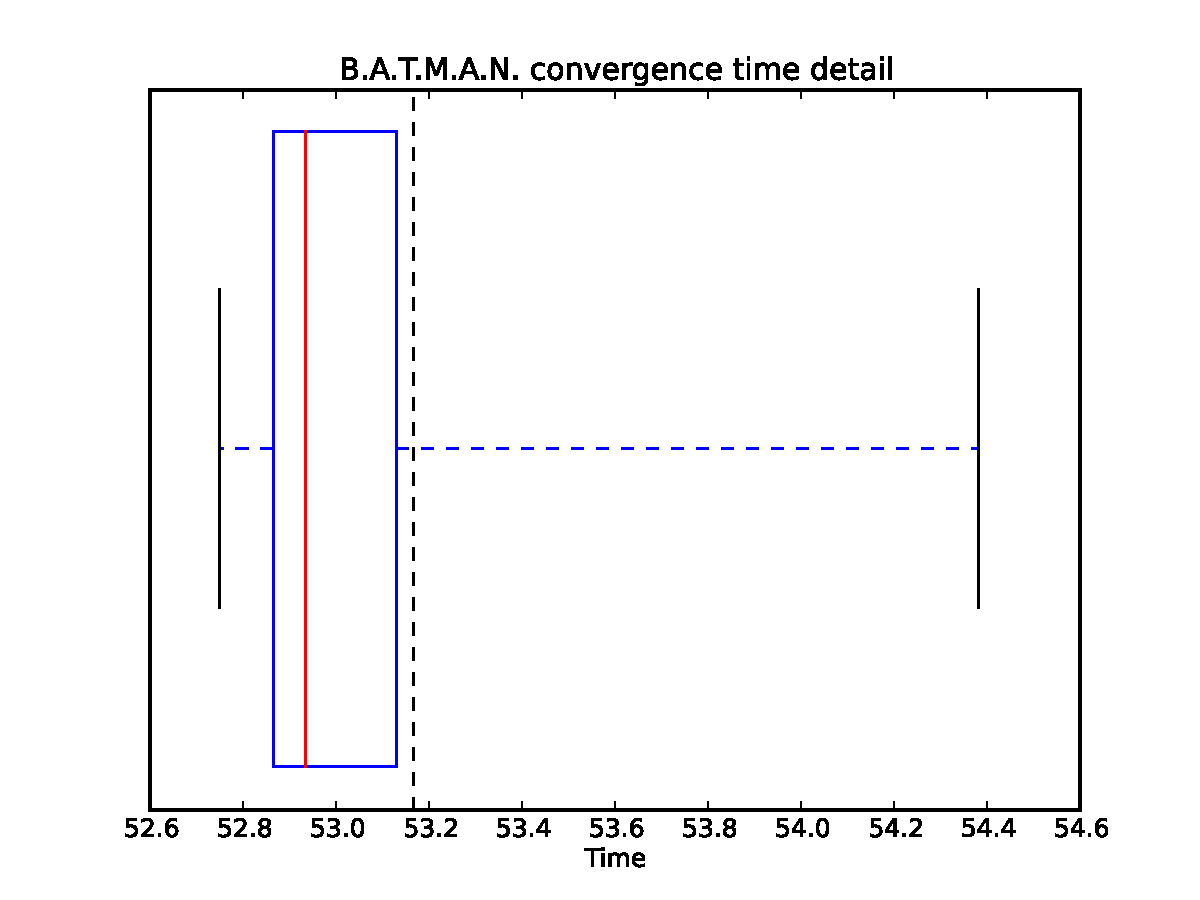
\includegraphics[width=\linewidth]{images/convergence_batman_plot_convergence_time}
    \caption{Detail of the convergence instant while using \batman\ as routing protocol}
    \label{pic:batman_convergence_time}
  \end{minipage}
  \hspace{0.5cm}
  \begin{minipage}[b]{0.5\linewidth}
    \centering
    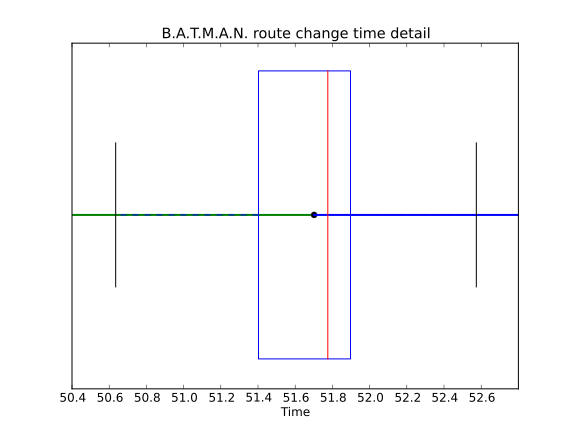
\includegraphics[width=\linewidth]{images/convergence_batman_plot_nexthop_change}
    \caption{Detail of the instant in which \batman\ changed the
                 preferred route}
    \label{pic:batman_convergence_change}
  \end{minipage}
\end{figure}


       \begin{table}[htbp]
            \centering
            \begin{tabular}{rccccccc}
            \toprule
            Kind & Average & Variance & Min & 1st Quartile &
            Median & 3rd Quartile & Max \\
            & \footnotesize{sec} & & \footnotesize{sec} & \footnotesize{sec} &
            \footnotesize{sec} & \footnotesize{sec} & \footnotesize{sec} \\
            \midrule
            Convergence & 13.166  & 0.250 & 12.749 & 12.856 & 12.935 & 13.149 &14.383\\
            Route change & 11.655 & 0.234 & 10.635 & 11.317 & 11.775 & 11.926 & 12.574\\
            \bottomrule
            \end{tabular}
            \caption{Statistics on the convergence and route change
              instants of \batman\ relative to the \emph{preferred
                route} kill time (i.e. second 40).}
            \label{tab:convergence_batman}
        \end{table}

\clearpage
\subsection{\olsr}
In this section are included the result for \olsr (see previous
subseciton for a description of the plot).
In Picture~\ref{pic:olsr_convergence} is shown the summary of our
test. A zoomed view of the convergence instant and next-hop change
instant is reported respectively in
Picture~\ref{pic:olsr_convergence_time}
and~\ref{pic:olsr_convergence_change}.


  \Picture{images/convergence_olsr_plot}
               {\textwidth}
               {Convergence plot while using \olsr\ as routing protocol}
               {pic:olsr_convergence}

\begin{figure}[bhtp]
  \begin{minipage}[b]{0.5\linewidth}
    \centering
    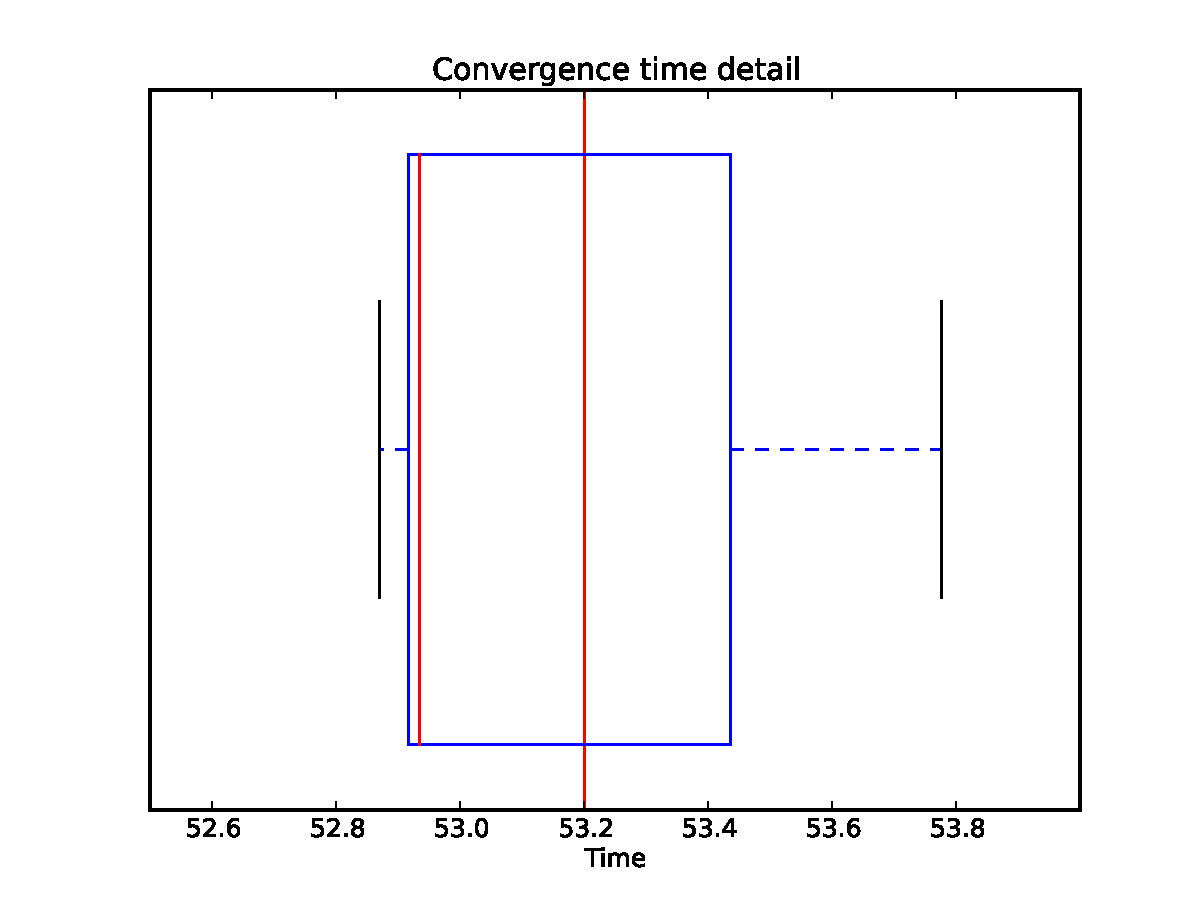
\includegraphics[width=\linewidth]{images/convergence_olsr_plot_convergence_time}
    \caption{Detail of the convergence instant while using \olsr\ as routing protocol}
    \label{pic:olsr_convergence_time}
  \end{minipage}
  \hspace{0.5cm}
  \begin{minipage}[b]{0.5\linewidth}
    \centering
    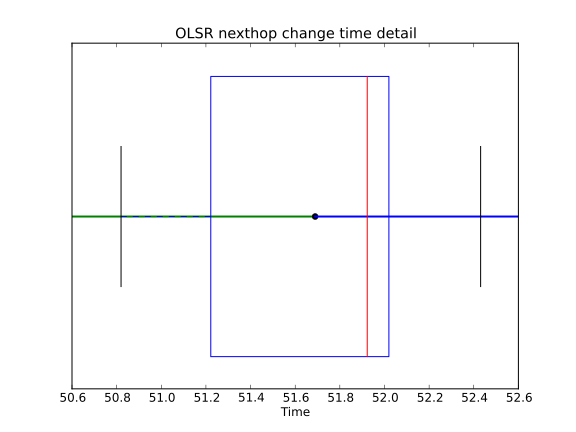
\includegraphics[width=\linewidth]{images/convergence_olsr_plot_nexthop_change}
    \caption{Detail of the instant in which \olsr\ changed the
                 preferred route}
    \label{pic:olsr_convergence_change}
  \end{minipage}
\end{figure}

       \begin{table}[htbp]
            \centering
            \begin{tabular}{rccccccc}
            \toprule
            Kind & Average & Variance & Min & 1st Quartile &
            Median & 3rd Quartile & Max \\
            & \footnotesize{sec} & & \footnotesize{sec} & \footnotesize{sec} &
            \footnotesize{sec} & \footnotesize{sec} & \footnotesize{sec} \\
            \midrule
            Convergence & 13.201 & 0.118 & 12.870 & 12.916 & 12.935 & 13.560 &13.776 \\
            Route change & 11.460 & 0.262 & 10.627 & 11.028 & 11.131 &11.827 & 12.238 \\
            \bottomrule
            \end{tabular}
            \caption{Statistics on the convergence and route change
              instants of \olsr\ relative to the \emph{preferred
                route} kill time (i.e. second 40).}
           \label{tab:convergence_olsr}
        \end{table}

\subsection{Consideration}

As can be easily seen by comparing Table~\ref{tab:convergence_batman}
with Table~\ref{tab:convergence_olsr}, the two mesh protocols
have almost equivalent performances: both show a
\emph{black out time} of about 13 seconds.

\begin{verbatim}
Such a similarity in the
results makes us think about a difference in the channel quality between
tests, rather than an actual differences in the protocol quality.

The results are so similar
which we didn't find any important aspect which cannot be attributed
to the mutated condition of the channel quality between tests.
\end{verbatim}

An interesting aspect which we discovered about both protocols is that
they employ a mechanism to discover missing paths, which goes
beyond the simple general flow of the protocol.

This is really easy to notice by looking at the output of \batman\ in
Listing~\ref{lst:batman_log}: we see that the
quality measure associated to node 10.0.0.66 (marked with a `*')
keep increasing until it goes abruptly to 0 (in the last block).
Interestingly at that
time such node was already down (this can be deduced by the fact that the
counter marked with `§' remains always the same).

\begin{figure}[tbhp]
\begin{Verbatim}[fontsize=\footnotesize]
...
 Originator  (#/255)         Nexthop [outgoingIF]:   Potential  nexthops ... [B.A.T.M.A.N. 0.3.2 ... ]
10.0.0.66       (206)       10.0.0.66 [      eth1]:       10.0.0.66 (206§)      10.0.0.68 ( 97)
10.0.0.67       (184)       10.0.0.66 [      eth1]:       10.0.0.66 (184*)      10.0.0.68 (138)
10.0.0.68       (192)       10.0.0.68 [      eth1]:       10.0.0.68 (192)       10.0.0.66 (124)

  Originator  (#/255)         Nexthop [outgoingIF]:   Potential nexthops ... [B.A.T.M.A.N. 0.3.2 ... ]
10.0.0.66       (206)       10.0.0.66 [      eth1]:       10.0.0.66 (206§)      10.0.0.68 ( 97)
10.0.0.67       (184)       10.0.0.66 [      eth1]:       10.0.0.66 (184*)      10.0.0.68 (140)
10.0.0.68       (199)       10.0.0.68 [      eth1]:       10.0.0.68 (199)       10.0.0.66 (126)

  Originator  (#/255)         Nexthop [outgoingIF]:   Potential nexthops ... [B.A.T.M.A.N. 0.3.2 ...]
10.0.0.66       (206)       10.0.0.66 [      eth1]:       10.0.0.66 (206§)      10.0.0.68 ( 97)
10.0.0.67       (185)       10.0.0.66 [      eth1]:       10.0.0.66 (185*)      10.0.0.68 (144)
10.0.0.68       (202)       10.0.0.68 [      eth1]:       10.0.0.68 (202)       10.0.0.66 (126)

  Originator  (#/255)         Nexthop [outgoingIF]:   Potential nexthops ... [B.A.T.M.A.N. 0.3.2 ...]
10.0.0.66       (206)       10.0.0.66 [      eth1]:       10.0.0.66 (206§)      10.0.0.68 ( 97)
10.0.0.67       (186)       10.0.0.66 [      eth1]:       10.0.0.66 (186*)      10.0.0.68 (146)
10.0.0.68       (207)       10.0.0.68 [      eth1]:       10.0.0.68 (207)       10.0.0.66 (  0)

  Originator  (#/255)         Nexthop [outgoingIF]:   Potential nexthops ... [B.A.T.M.A.N. 0.3.2 ...]
10.0.0.66       (206)       10.0.0.66 [      eth1]:       10.0.0.66 (206§)      10.0.0.68 ( 97)
10.0.0.67       (150)       10.0.0.68 [      eth1]:       10.0.0.66 (  0*)      10.0.0.68 (150)
10.0.0.68       (211)       10.0.0.68 [      eth1]:       10.0.0.68 (211)       10.0.0.66 (  0)
...
\end{Verbatim}
\caption{Snippet of \batman\ output}
\label{lst:batman_log}
\end{figure}

A similar thing happens also in \olsr: the link to node 10.0.0.66 is
maintained with a better quality measure but it is abruptly removed
from the 2-hop list for node 10.0.0.67 (see Listings~\ref{lst:olsr_log}).

\begin{figure}[tbhp]
\begin{Verbatim}[fontsize=\footnotesize]
...
--- 11:20:20.930522 ---------------------------------------------------- LINKS

IP address       hyst         LQ       ETX
10.0.0.68        0.000  0.482/0.576    3.596
10.0.0.66        0.000  0.729/0.765    1.793

--- 11:20:20.930547 ----------------------- TWO-HOP NEIGHBORS

IP addr (2-hop)  IP addr (1-hop)  Total cost
10.0.0.67        10.0.0.66        2.641
                 10.0.0.68        4.680
...
--- 11:20:21.030784 ---------------------------------------------------- LINKS

IP address       hyst         LQ       ETX
10.0.0.68        0.000  0.482/0.576    3.596
10.0.0.66        0.000  0.729/0.765    1.793

--- 11:20:21.030836 ----------------------- TWO-HOP NEIGHBORS

IP addr (2-hop)  IP addr (1-hop)  Total cost
10.0.0.67        10.0.0.68        4.680
...
\end{Verbatim}
\caption{Snippet of \olsr\ output}
\label{lst:olsr_log}
\end{figure}

Given this behavior, our hypothesis is that the quality of the link
should not influence the convergence time.
